\chapter{The Large Hadron Collider}
The Large Hadron Collider (LHC) is a 27km long circular particle accelerator, located 100m underground near the city of Geneva, Switzerland and spanning the border of France and Switzerland. The LHC is operated by the  European Organization for Nuclear Research (CERN), the largest international scientific collaboration in the world. The LHC uses the same tunnel employed by the former Large-Electron-Positron Collider (LEP), as well as some of the LEP infrastructure as part of it's injection chain.\\

The LHC accelerates protons and heavy ions and collides them at four interaction points around the ring, with a design center-of-mass energy per collision of $\sqrt{s}$ = 14 TeV. Each interaction point is home to one of four detector experiments, which study the products of the collisions. The largest of these experiments is the $ATLAS$ detector, a general purpose detector for studying the SM and searching for physics beyond it. The $CMS$ detector is another general purpose detector, designed and operated independently of the $ATLAS$ detector, but intended to probe the same range of physics. The $ALICE$ experiment is a dedicated heavy ion experiment, and the $LHC-b$ experiment is a dedicated $b$-physics experiment.\\

 \section{Accelerator Physics}
 \subsection{The Journey of a Proton}
 Protons which feed the LHC start as hydrogen gas. The electrons are removed from the hydrogen atoms through the use of strong electric fields. The linear accelerator (LINAC) then accelerates the $H^-$ ions to an energy of 50 MeV. From here the $H^-$ ions enter the Proton Synchrotron booster, where they are accelerated up to 1.4 GeV of energy. Subsequently they pass through the Proton Synchroton (PS) and the Super Proton Synchrotron (SPS), where they reach energies of 25 GeV and 450 GeV respectively. Finally they are injected into the LHC as two beams traveling in opposite direction, and can be accelerated up to 7 TeV of energy. Due to limitations with the magnet training, the highest energy actually achieved by the LHC beams during Run 2 was 6.5 TeV each, giving a collision center-of-mass energy of $\sqrt{s}$ = 13 TeV. Figure \ref{fig:accelerator_complex} shows the full LHC accelerator complex.\\

\begin{figure}
	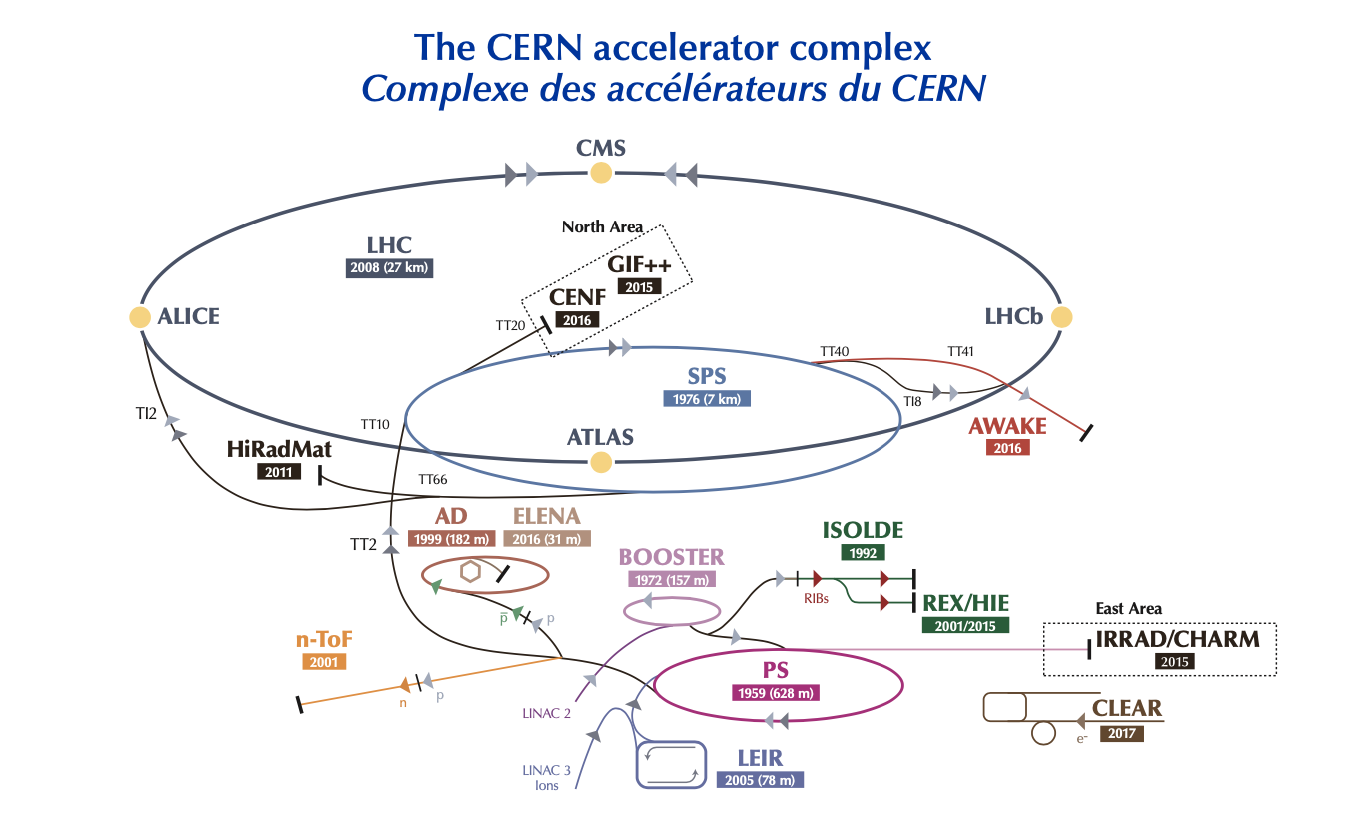
\includegraphics[width=\textwidth]{figures/accelerator_complex.png}
	\caption{The LHC accelerator complex at CERN}
	\label{fig:accelerator_complex}
\end{figure}

 Acceleration in the LHC is performed by eight radio frequency cavities located around the ring. 
 
 Bunches\\ 
 
 Luminosity